%%%%%%%%%%%%%%%%%%%%%%%%%%%%%%%%%%%%%%%
%                                     %
%   %    %   %  %   %%%%%    %  %  %  %
%  %%   %%   %  %   %       %%  %  %  %
%   %    %   %%%%%  %%%%%    %  %%%%% %
%   %    %      %       %    %     %  %
%  %%%  %%%     %   %%%%%   %%%    %  %
%                                     %
%%%%%%%%%%%%%%%%%%%%%%%%%%%%%%%%%%%%%%%

%本实验报告由本人林诚皓和吉骏雄一起完成, 旨在方便LATEX原教旨主义者写实验报告, 避免Word文档因插入过多图造成卡顿. 

\documentclass[11pt]{article}

\usepackage[a4paper]{geometry}
\geometry{left=2.0cm,right=2.0cm,top=2.5cm,bottom=2.5cm}

\usepackage{ctex}
\usepackage{amsmath,amsfonts,graphicx,subfigure,amssymb,bm,amsthm}
\usepackage{algorithm,algorithmicx}
\usepackage[noend]{algpseudocode}
\usepackage{fancyhdr}
\usepackage{mathrsfs}
\usepackage{mathtools}
\usepackage[framemethod=TikZ]{mdframed}
\usepackage{fontspec}
\usepackage{adjustbox}
\usepackage{breqn}
\usepackage{fontsize}
\usepackage{tikz,xcolor}
\usepackage{multirow} 
\usepackage{booktabs}
\usepackage{tcolorbox}
\usepackage{pdfpages}
\setmainfont{Palatino Linotype}
\setCJKmainfont{SimHei}
\setCJKsansfont{Songti}
\setCJKmonofont{SimSun}
\punctstyle{kaiming}

\renewcommand{\emph}[1]{\begin{kaishu}#1\end{kaishu}}

%改这里可以修改实验报告表头的信息
\newcommand{\experiName}{微波布拉格衍射}
\newcommand{\supervisor}{刘荣鹃}
\newcommand{\name}{李果}
\newcommand{\studentNum}{2022K8009906028}
\newcommand{\class}{01}
\newcommand{\group}{09}
\newcommand{\seat}{8}
\newcommand{\dateYear}{2023}
\newcommand{\dateMonth}{11}
\newcommand{\dateDay}{13}
\newcommand{\room}{717}
\newcommand{\others}{$\square$}
%% 如果是调课、补课, 改为: $\square$\hspace{-1em}$\surd$
%% 否则, 请用: $\square$
%%%%%%%%%%%%%%%%%%%%%%%%%%%

\begin{document}

%若需在页眉部分加入内容, 可以在这里输入
% \pagestyle{fancy}
% \lhead{\kaishu 测试}
% \chead{}
% \rhead{}

\begin{center}
    \LARGE \bf 《\, 基\, 础\, 物\, 理\, 实\, 验\, 》\, 实\, 验\, 报\, 告
\end{center}

\begin{center}
    \noindent \emph{实验名称}\underline{\makebox[25em][c]{\experiName}}
    \emph{指导教师}\underline{\makebox[8em][c]{\supervisor}}\\
    \emph{姓名}\underline{\makebox[6em][c]{\name}}%%如果名字比较长, 可以修改box的长度"5em"
    \emph{学号}\underline{\makebox[10em][c]{\studentNum}}
    \emph{分班分组及座号} \underline{\makebox[5em][c]{\class \ -\ \group \ -\ \seat }\emph{号}} (\emph{例}:\, 1\,-\,04\,-\,5\emph{号})\\
    \emph{实验日期} \underline{\makebox[3em][c]{\dateYear}}\emph{年}
    \underline{\makebox[2em][c]{\dateMonth}}\emph{月}
    \underline{\makebox[2em][c]{\dateDay}}\emph{日}
    \emph{实验地点}\underline{{\makebox[4em][c]\room}}
    \emph{调课/补课} \underline{\makebox[3em][c]{\others\ 是}}
    \emph{成绩评定} \underline{\hspace{5em}}
    {\noindent}
    \rule[8pt]{17cm}{0.2em}
\end{center}

\begin{center}
\LARGE{微波布拉格衍射}
\end{center}

\tableofcontents

% \listoffigures
% \listoftables

\newpage
\section{实验目的}

1.了解与学习微波的基本特性、产生基本原理以及传播和接收等基本性质。

2.观测微波衍射、干涉等实验现象。

3.观测模拟晶体的微波布拉格衍射现象(110面和100面)。

4.通过迈克耳逊实验测量微波波长。

5.了解并检验光偏振的马吕斯定律。

\section{实验器材}

DHMS-1 型微波光学综合实验仪一套,
以及其他的实验用件(反射板、分束板、单缝板、双缝板、晶体模型等)。
具体可以详见图1。

\begin{figure}[H]
    \centering
    \includegraphics[width=8cm]{图1.jpg}
    \caption{1.X 波段信号源 2.固定臂 3.长支柱 4.紧固蝶形螺丝 5.信号源传输电缆
6.频率调节旋钮 7.功率调节旋钮 8.发射器喇叭 9.指针 
10.载物圆台 11.圆形支架 12.短支柱 13.接收器喇叭
14.接收旋转部件 15.接收器信号输出插座 16.检流计调零电位器
17.检流计电源开关 18.检流计信号输入插座 19.转动臂 20.紧固螺杆
21.移动装置 22.圆形底盘 23.水平调节机脚 24.模拟晶格
25.玻璃板 26.反射板 27.单缝板 28.双缝板}
\end{figure}








\section{实验原理}

\subsection{微波的产生与接收}

本实验使用的微波发生器是采用电调制方法实现的:
简单来说,就是利用微波发生器内部的一个电压可调控制的VCO,
产生一个4.4GHz-5.2GHz的信号,
经过滤波器后取二次谐波8.8GHz-9.8GHz,
再经过衰减器、放大器、隔离器后,
通过探针输出至波导口,再通过E面天线发射出去。
其工作原理见图2。

接收部分采用检波/数显一体化设计。
可将接收到的微波转化为电信号并显示在液晶屏上。

\begin{figure}[H]
    \centering
    \includegraphics[width=10cm]{图2.jpg}
    \caption{微波的产生原理}
\end{figure}

\subsection{微波双缝衍射实验}

两条缝分别发出的次级波有稳定相位差(且频率和振动方向一致),是相干波,故会产生干涉现象。
此外,实验将是衍射和干涉两者结合的结果。
令双缝的缝宽$a$接近$\lambda$(这样能衍射现象较为明显),当两条缝之间的间隔$b$较大时,
干涉强度受单缝衍射的影响小,当$b$较小时,
干涉强度受单缝衍射影响大。

干涉加强的角度为:
\begin{displaymath}\theta=\arcsin \frac{k\lambda}{a+b}\qquad \text{ 对应波长 }\lambda=\frac{a+b}{k}\sin \theta\end{displaymath}
干涉减弱的角度为:
\begin{displaymath}\theta=\arcsin \frac{\frac{2k+1}\lambda}{a+b} \qquad \text{ 对应波长 }\lambda=\frac{a+b}{\frac{2k+1}{2}} \sin \theta\end{displaymath}

\subsection{微波的迈克尔逊干涉实验}

在微波前进的方向上放置一个与波传播方向成45°角的半透射
半反射的分束板,它将入射波分成一束向反射板A传播,
另一束向反射板B传播。
这两束微波经过一系列透射和反射后,
将在在接收器处发生干涉,
干涉叠加的强度由两束波的程差决定。
当两波的相位差为$2k\pi,\pi\in\mathbb{Z}$ 时,
为干涉极强,相位差为$(2k+1)\pi$时,为干涉极小。

固定其中一个金属板(本实验装置固定的是反射板A),
移动另一块(即反射板B),当连续两次达到极大值(或极小值)时,
反射板移动了半波长$\displaystyle\frac{\lambda}{2}$,
由此可知,第$n$次达到极大值(或极小值)时,若金属板移动了$L$,
则有关系式:
\begin{displaymath}\lambda=\frac{2L}{n}\end{displaymath}


\subsection{微波布拉格衍射}

组成晶体的原子或分子按一定规律在空间周期性排列。
其中最简单的结构,原子在空间中按固定的距离$a$在空间依序重复排列而形成的简单立方点阵,
如下图3所示,
原子间距$a$称为晶格常数。
晶面即组成晶体的原子处在的一系列相互平行而且间距一定的平面族,
常见的(也是本次实验需要做的),
是$(100)$和$(110)$两种结构。

根据刘老师ppt,:
晶面在$x,y,z$坐标轴上截距的倒数化为最小整数后的值记为$h,k,l$,
也常被称作晶面指数,用以表征所取的晶面方向和形状,
则相邻的两个晶面间距为:
\begin{displaymath}d=\frac{a}{\sqrt{h^2+k^2+l^2}}\end{displaymath}

常见的几种晶格类型可由下图所示,其中圆括号括起来的三个数分别表示$(hkl)$。
\begin{figure}[H]
    \centering
    \includegraphics[width=7cm]{图4.jpg}
    \caption{不同晶面结构}
\end{figure}

电磁波入射到晶体要受到晶体的衍射,如今我们要考察的小孔是三维空间中原子组成的格点,是一个三维的光栅网络。

\begin{figure}[H]
    \centering
    \includegraphics[width=8cm]{图5.jpg}
    \caption{左图为同一个晶面的散射波示意图,而右图是不同晶面的散射波示意图}
\end{figure}

散射波的反射角等于入射角,如上图5所示,再相干叠加
而从间隔为$d$的相邻两个晶面反射的两束波的程差为$2d\sin \theta$,$\theta$
为入射角与晶面的夹角.

可以看见,形成干涉极大的方程为:
$$2d\sin \theta=k\lambda,k\in\mathbb{Z}$$

该方程被称为晶体衍射的布拉格条件.

如果布拉格条件得到满足,
每一个晶面族在特定方向产生一个衍射极大,
从实验上测得衍射极大的方向角$\beta$,
并且知道波长$\lambda$,从布拉格条件可求出晶面间距$d$,
通过进一步分析可以确定$d$、晶格常数$a$、波长$\displaystyle\lambda=\frac{2d\cos \beta}{k}$


\subsection{微波的偏振实验(选做)}

% \begin{figure}[H]
%     \centering
%     \includegraphics[width=6cm]{图6.jpg}
%     \caption{马吕斯定律}
% \end{figure}

% 其本质还是光学中的马吕斯定律。

\subsection{微波单缝衍射实验(选做)}

*这两部分为选做实验,将在后续实验数据处理部分详细讨论。


\section{实验内容概要}

1. 测量微波的双缝干涉强度分布,从而计算微波的波长;

2. 观察并测量晶面为100面和110面的布拉格衍射现象。从而得到布拉格角度和晶格常数,计算微波波长;

3. 利用迈克尔逊干涉实验装置,观察干涉现象并记录极小值位置,计算微波的波长;

4.(选做)微波单缝衍射实验与检验马吕斯定律;

5.对上述数据进行误差分析和总结归纳,并与频谱分析仪测量的波长结果做比较。

\bigskip
其中具体的一些实验操作细节、实验注意点和其中我的心得收获,我会在下面每一小节中穿插叙述。

\newpage
\section{实验结果与数据处理}

\subsection{实验前的准备}

\subsubsection{调平、对直与预热}

按照实验讲义的要求,进行以下三个步骤:

·调平:将实验仪器放置在水平桌面上,
调整底座四只脚使底盘保持水平。

·对直:调节保持发射喇叭、接收喇叭、接收臂、活动臂为直线对直状态,
并且调节发射喇叭,接收喇叭的高度相同,角度相同且长轴边都平行于桌面。

·预热:连接好 X 波段微波信号源、微波发生器间的专用导线,
将微波发生器的功率调节旋钮逆时针调到底,
即微波功率调至最小,通电并预热 10 分钟。

·其他调整:适当挪动实验装置,使得动臂相对微波发生器能有正负50°的旋转区域,便于后续实验;适当摆放桌上物品与装置,使得它们对微波信号的测量影响尽可能小。

实际实验过程中,最开始就可打开微波发生器,利用玻璃板等辅助工具对直和调平试验仪后,再调准微波发射频率后,预热过程就可视为完成。


\subsubsection{实验条件确认}

本实验采用的实验条件为:$f=9.4$GHz

根据查阅到的微波发生器侧面表格的数据,调节左侧旋钮,
此时所对应的理论波长$\lambda=c/f\approx 3.1893\,\, \rm {cm}$

下图是我调制的结果:

\begin{figure}[H]
    \centering
    \includegraphics[width=10cm]{IMG_20231113_142444.jpg}
    \caption{微波频率调制结果}
\end{figure}


\subsubsection{每个试验前的仪器对准确认}

在本次实验中,我们和数学通用规范采同样标准:
即以顺时针方向(即实验台朝外方向)为负角度,逆时针
方向(即实验台朝内方向)为正角度。例如,上表中的-20°指以 0°刻线为基准线,视线正对表盘,
以表盘正中心为圆心,顺时针旋转 20°所得的角度位置。

实验之前,我将讲义大致读了一遍,
细致完成了预习实验报告的要求和撰写。
通过实验简介大致了解了微波的相关知识,
了解了微波的产生与接收原理(因为后续采用一体化的实验设备,故没有继续探究下去)
后,了解了布拉格晶体的衍射的相关知识(我先在原子物理课程上学习到了这一概念)等等,对我做实验也是很有帮助的。
在正式做实验之前,刘老师强调了一点是我觉得比较有趣的:晶体的晶格常数量级很小,需要用同等量级的 X 射线波才能观察到衍射现象。然而
如果利用小球模型模拟晶体结构,用微波就可以观察到衍射现象,并且由相同的公式支
配。也就是说厘米量级波长应该对应厘米量级的晶体。

在了解实验基本知识和操作流程之后,
我还计算出各个子实验测量量的理论值——用以辅助实验,
判断实验数据的可靠性和自己操作的正确性。
其中双缝缝宽$a=3.5$cm,缝之间的间距$b=5$cm;布拉格衍射实验中面间距$d=4$cm;单缝衍射实验中缝宽$p=8$cm。
并制作成下面的表:

\begin{table}[H]
    \centering
    \begin{tabular}{cccc}
        \toprule
        \multicolumn{4}{c}{理论波长:$\lambda =3.1893$cm}  \\ 
        \midrule
        实验名称 &测量范围&理论角度计算公式&理论角度值(°)\\
        \midrule
        \multirow{3}*{微波双缝干涉} & 一级极大 &$\arcsin \cfrac{\lambda}{a+b}$  & 22.03740 \\ 
           & 零级极小 & $\arcsin \cfrac{\lambda}{2(a+b)}$& 10.81310 \\ 
           & 一级极小 &$\arcsin \cfrac{3\lambda}{2(a+b)}$ & 34.25088 \\ 
        \midrule
        \multirow{2}*{布拉格衍射}& (100)晶面 & $\arccos\cfrac{\lambda}{2d}$ & 66.50541 \\ 
            &(110)晶面 &  $\arccos\cfrac{\lambda}{\sqrt 2 d}$  & 55.68142 \\ 
        \midrule
        微波单缝衍射 & 极小值处 & $\arcsin \cfrac{\lambda}{p}$ & 23.49459 \\ 
        \bottomrule
    \end{tabular}
    \caption{微波实验:部分子实验理论角度值}
\end{table}

在实验过程中,为了尽可能减小实验误差,在每次子实验之前我都耐心仔细地做了微波仪器的对准确认环节(反复调整在正负20°处,并微调接收器方向和角度,使得两点测量到的信号强度差不超过0.2mV)。将对准的结果汇总为以下的表:

\begin{table}[!ht]
    \centering
    \begin{tabular}{ccccc}
    \toprule
        \multirow{2}*{实验名称$\backslash$电压(mV)} & \multicolumn{3}{c}{角度(°)}  & \multirow{2}*{差值} \\ 
        \cmidrule(lr){2-4}
        & -20 & 0 & 20   \\ \midrule
        双缝干涉实验 & 15.8 & 177.7 & 15.9 & 0.1 \\ 
        微波迈克尔逊干涉实验 & 15.8 & 173.3 & 15.9 & 0.1 \\ 
        微波布拉格衍射实验(100晶面) & 11.2 & 148.6 & 11.4 & 0.2 \\ 
        微波布拉格衍射实验(110晶面) & 10.0 & 139.0 & 10.1 & 0.1 \\ 
        微波单缝衍射实验 & 14.3 & 165.8 & 14.4 & 0.1 \\ 
        微波的偏振实验 & 12.9 & 155.8 & 12.8 & -0.1 \\ 
        \bottomrule
    \end{tabular}
    \caption{微波实验仪对准确认:数据一览表}
\end{table}


微波试验仪的对准操作在后续实验部分中不再赘诉。

实验过程中还发生了一个小插曲:
当我测量完布拉格衍射实验中(100)晶面的数据时,发现偏差比预期要大。
通过对前期计算的理论角度值的查询以及和刘老师的讨论确认,初步判断为实验过程中记录小角度数据时,触碰到微波发生器而导致实验的不成功。
这一方面提醒我测量(110)晶面时需要重新对准确认,最终获得了不错的结果(见下面数据处理);另一方面也体现了前期预习、准备等工作的必要性。










\newpage

\subsection{双缝干涉实验}

按需要调整双缝干涉板的缝宽$a=3.5$cm,缝间距则测量为$b=5$cm。
将双缝缝干射板安置在支座上时,
应使双缝板平面与载物圆台上90度指示线一致。
转动小平台使固定臂的指针在小平台的180度处。
此时相当于微波从双缝干涉板法线方向入射。
这时让活动臂置小平台0度处,
调整信号使液晶显示器显示较大(否则可能导致极小值处数据记录困难,无法分辨)。

在0度线的两侧,每改变2度读取一次液晶显示器的读数(实验过程中我采用了先记录完全一侧数据,再换至另一侧,尽量减小移动动臂时对微波接受器的影响),
并记录下来,然后画出双缝干涉强度与角度的关系曲线。并根据微波衍射强度图像中的特征范围,确定下一步细扫操作的角度区域。并最终结合缝宽$a$与缝间距$b$,计算微波波长$\lambda$及其百分误差。

在这实验之前,我先做了一个“预实验”:
转动接收器,确认其可以在需要测的0°到正负50°范围内自由转动不受阻碍,并且读数不至过
大或过小。这么做的理由,一是为了防止出现转动接收器时受阻碍的情况,二是为了防止出
现扫描过程中出现超量程(过大或过小)的情况。之后开始正式实验,
我记录到的原始实验数据如下表:
\begin{table}[H]
    \centering
    \begin{tabular}{cccccccccccccc}
    \toprule
        角度$\theta$(°) & 0 & 2 & 4 & 6 & 8 & 10 & 12 & 14 & 16 & 18 & 20 & 22 & 24 \\ \midrule
        $U_{\theta+}$(mV) & 37.5  & 39.2  & 31.8  & 25.0  & 15.2  & 3.3  & 0.0  & 0.2  & 2.0  & 8.2  & 20.2  & 35.6  & 43.2  \\ 
       $U_{\theta-}$(mV)& 37.6  & 26.8  & 9.9  & 1.1  & 0.3  & 1.0  & 4.6  & 14.3  & 32.5  & 42.3  & 39.0  & 24.2  & 10.6  \\ 
       \bottomrule \toprule
        角度(°) & 26 & 28 & 30 & 32 & 34 & 36 & 38 & 40 & 42 & 44 & 46 & 48 & 50 \\ \midrule
        $U_{\theta+}$(mV) & 37.3  & 22.2  & 6.4  & 2.0  & 0.6  & 0.3  & 0.6  & 1.6  & 1.9  & 0.8  & 0.5  & 2.9  & 5.0  \\ 
        $U_{\theta-}$(mV) & 2.4  & 1.5  & 2.8  & 6.5  & 10.5  & 7.3  & 1.9  & 0.6  & 3.9  & 10.9  & 8.2  & 1.3  & 0.2 \\ \bottomrule
    \end{tabular}
    \caption{双缝干涉实验:粗扫实验数据}
\end{table}

由此做出粗扫图像:

\begin{figure}[H]
    \centering
    \includegraphics[width=12cm]{1 粗.png}
    \caption{双缝干涉实验:粗扫实验数据制图}
\end{figure}


可以看到,实际结果并不是特别理想:

·首先是原点处不是极大值点,在原点附近的性状也比较奇怪。
而且有些许遗憾地是,当时并没有补测1°方向的实验数据,按照图像趋势,可能这一角度才是真正的“最大值”。

·整体看来,其对称性也不是很好——图像整体向正方向偏差了2°左右。
两侧极大值、极小值的峰值强度也不是很对称。

·在角度过大时的规律也不够明显。


\newpage
但是整体来说,这个图像还是能够反映双缝干涉的情况的。现在根据实验数据,再做更细一步的研究:

大致可以看出:双缝干涉的一级极大大约在(+20°,+28°)、(-22°,-14°)范围;
零级极小大约在(+8°,+16°)、(-12°,-4°)范围;
一级极小大约在(+32°,+40°)、(-33°,-25°)范围。
于是保持功率不变,以1度角为间隔进行细扫,得到数据如下:
\begin{table}[H]
    \centering
    \begin{tabular}{ccccccccccccc}
    \toprule
        \multirow{2}*{数据点} & \multicolumn{4}{c}{一级极大} &\multicolumn{4}{c}{ 零级极小}  & \multicolumn{4}{c}{一级极小 }\\ 
        \cmidrule(lr){2-5}  \cmidrule(lr){6-9}  \cmidrule(lr){10-13}
        & $\theta$ & $U_{\theta+}$(mV) & $\theta$  &$U_{\theta-}$(mV)& $\theta$  & $U_{\theta+}$(mV) & $\theta$  &$U_{\theta-}$(mV) & $\theta$  & $U_{\theta+}$(mV) & $\theta$  & $U_{\theta-}$(mV) \\ \midrule
        1 & 20 & 20.1 & 14 & 14.8 & 8 & 14.6  & 4 & 10.3 & 32 & 1.9 & 25 & 4.9 \\ 
        2 & 21 & 28.4 & 15 & 22.3 & 9 & 8.0  & 5 & 3.3 & 33 & 1.1 & 26 & 2.2 \\ 
        3 & 22 & 35.2 & 16 & 32.9 & 10 & 3.0  & 6 & 1.1 & 34 & 0.7 & 27 & 1.4 \\ 
        4 & 23 & 39.8 & 17 & 38.1 & 11 & 0.4  & 7 & 0.4 & 35 & 0.4 & 28 & 1.5 \\ 
        5 & 24 & 42.3 & 18 & 41.9 & 12 & 0.0  & 8 & 0.3 & 36 & 0.3 & 29 & 2.1 \\ 
        6 & 25 & 40.8 & 19 & 42.5 & 13 & 0.1  & 9 & 0.5 & 37 & 0.2 & 30 & 3.0  \\ 
        7 & 26 & 36.7 & 20 & 38.9 & 14 & 0.2  & 10 & 1.1 & 38 & 0.5 & 31 & 4.6 \\ 
        8 & 27 & 30.4 & 21 & 31.4 & 15 & 0.6  & 11 & 2.1 & 39 & 0.9 & 32 & 6.2 \\ 
        9 & 28 & 21.3 & 22 & 23.7 & 16 & 1.8  & 12 & 4.2 & 40 & 1.5 & 33 & 8.6 \\ \bottomrule
    \end{tabular}
    \caption{双缝干涉实验:细扫实验数据(一级极大、零级极小和一级极小)}
\end{table}

根据一级极大的正负两侧数据,做出图像,并导入Get Data软件进行数据读取(见右上角,x坐标值即为紫色点对应的角度值),尽可能减少人为读取造成的二次误差。

\begin{figure}[H]
    \centering
    \subfigure[数据制图]{\includegraphics[height=7cm]{1 11.png}}\hspace{0.5cm}
    \subfigure[读取数据]{\includegraphics[height=7cm]{1 一级极大正.png}}
    \caption{双缝干涉实验:一级极大附近精细曲线(正角度)}
\end{figure}

\begin{figure}[H]
    \centering
    \subfigure[数据制图]{\includegraphics[height=6.5cm]{1 1 -1.png}}\hspace{0.5cm}
    \subfigure[读取数据]{\includegraphics[height=6.5cm]{1 一级极大负.png}}
    \caption{双缝干涉实验:一级极大附近精细曲线(负角度)}
\end{figure}

故而一级极大对应的正负角度值约为
\[
   \theta_+=24.0791^{\circ}\qquad\theta_{-}=18.7580^{\circ} 
\]
考虑整体干涉图像有$\theta_0=2°$的偏移,计算得到波长为:
\[
   \lambda_+=(a+b)\sin {(\theta_+-\theta_0)}\approx 3.1950\,\,{\rm cm}\qquad 
   \lambda_+=(a+b)\sin {(\theta_{-}+\theta_0)}\approx 3.0126\,\,{\rm cm}
\]
计算误差,分别为:
\begin{displaymath}
    \eta_+=\frac{|\lambda_+-\lambda_0|}{\lambda_0}=0.18\%\qquad
    \eta_{-}=\frac{|\lambda_{-}-\lambda_0|}{\lambda_0}=5.54\%
\end{displaymath}
对于实验数据评价和误差分析,在本节“实验总结”部分,我会统一叙述。

\bigskip
同理,根据零级极小的正负两侧数据,做出图像,并导入Get Data软件进行数据读取:
% \begin{figure}[H]
%     \centering
%     \subfigure[数据制图]{\includegraphics[height=7cm]{}}\hspace{0.5cm}
%     \subfigure[读取数据]{\includegraphics[height=7cm]{}}
%     \caption{双缝干涉实验:级极附近精细曲线(角度)}
% \end{figure}

\begin{figure}[H]
    \centering
    \subfigure[数据制图]{\includegraphics[height=7cm]{1 01.png }}\hspace{0.5cm}
    \subfigure[读取数据]{\includegraphics[height=7cm]{1 零级极小正.png}}
    \caption{双缝干涉实验:零级极小附近精细曲线(正角度)}
\end{figure}

\begin{figure}[H]
    \centering
    \subfigure[数据制图]{\includegraphics[height=7cm]{1 0 -1.png}}\hspace{0.5cm}
    \subfigure[读取数据]{\includegraphics[height=7cm]{1 零级极小负.png}}
    \caption{双缝干涉实验:零级极小附近精细曲线(负角度)}
\end{figure}


故而零级极小对应的正负角度值约为
\[
   \theta_+=12.3341^{\circ} \qquad\theta_{-}=8.06497^{\circ} 
\]
考虑整体干涉图像有$\theta_0=2^{\circ}$的偏移,计算得到波长为:
\[
   \lambda_+=2(a+b)\sin {(\theta_+-\theta_0)}\approx 3.0496\,\,{\rm cm}\qquad 
   \lambda_+=2(a+b)\sin {(\theta_{-}+\theta_0)}\approx 2.9710\,\,{\rm cm}
\]
计算误差,分别为:
\begin{displaymath}
    \eta_+=\frac{|\lambda_+-\lambda_0|}{\lambda_0}=4.38\%\qquad
    \eta_{-}=\frac{|\lambda_{-}-\lambda_0|}{\lambda_0}=6.84\%
\end{displaymath}





\bigskip
对于一级极小的数据处理是很类似的:
根据一级极小的正负两侧数据,做出图像,并导入Get Data软件进行数据读取。

\begin{figure}[H]
    \centering
    \subfigure[数据制图]{\includegraphics[height=6.5cm]{1 -1 1.png}}\hspace{0.5cm}
    \subfigure[读取数据]{\includegraphics[height=6.5cm]{1一级极小正.png}}
    \caption{双缝干涉实验:一级极小附近精细曲线(正角度)}
\end{figure}

\begin{figure}[H]
    \centering
    \subfigure[数据制图]{\includegraphics[height=7cm]{1 -1 -1.png}}\hspace{0.5cm}
    \subfigure[读取数据]{\includegraphics[height=7cm]{1 一级极小负.png}}
    \caption{双缝干涉实验:一级极小附近精细曲线(负角度)}
\end{figure}



故而一级极小对应的正负角度值约为
\[
   \theta_+=36.8936^{\circ}\qquad\theta_{-}=27.4074^{\circ} 
\]
考虑整体干涉图像有$\theta_0=2°$的偏移,计算得到波长为:
\[
   \lambda_+=\frac{2}{3}(a+b)\sin {(\theta_+-\theta_0)}\approx 3.2416\,\,{\rm cm}\qquad 
   \lambda_+=\frac{2}{3}(a+b)\sin {(\theta_{-}+\theta_0)}\approx 2.7824\,\,{\rm cm}
\]
计算误差,分别为:
\begin{displaymath}
    \eta_+=\frac{|\lambda_+-\lambda_0|}{\lambda_0}=1.64\%\qquad
    \eta_{-}=\frac{|\lambda_{-}-\lambda_0|}{\lambda_0}=12.76\%
\end{displaymath}



\begin{center}
    \begin{tcolorbox}[colback=gray!10,%gray background
                      colframe=black,% black frame colour
                      width=5cm,% Use 8cm total width,
                      arc=1mm, auto outer arc,
                      boxrule=0.5pt,
                     ]
                     \begin{center}
                    微波双缝干涉:实验总结      
                     \end{center}
    \end{tcolorbox}
\end{center}


先将上述计算得到的波长与误差进行汇总,并制作成下表:
\begin{table}[H]
    \centering
    \begin{tabular}{ccc|cc}
        \toprule
        数据来源区域 & $\lambda_+$(cm) & 误差 & $\lambda_{-}$(cm) & 误差 \\ 
        \midrule
        一级极大 & 3.1950 & 0.18\% & 3.0126 & 5.54\% \\ 
        零级极小 & 3.0496 & 4.38\% & 2.9710 & 6.84\% \\ 
        一级极小 & 3.2416 & 1.64\% & 2.7824 & 12.76\% \\ 
        \bottomrule
    \end{tabular}
    \caption{微波双缝干涉实验:计算结果一览表}
\end{table}

从中可以发现:

·正角度测量的数据总是比负角度的更为精准。原因可能是正角度(实验台朝内)是在海绵尖劈的包围下,后者起到了一定的屏蔽作用。
而负角度朝向外侧,在实验过程中难免会受到人员移动(我在移动过程中示数都会发生变化)或其他台桌的干扰等,故而其数据精度较低。

·一级极小的负角度测量误差达到了12.76\%,算是实验失误。其原因可能是,该角度最靠外,
而微波试验仪的对准与否的精细差别、
其他主要误差来源的影响都会在较大角度显著体现。

·综合来看,一级极大的实验计算结果最精确,
而零级极小、一级极小实验数据偏差稍大。

总体而言,这次的双缝干涉实验还是较为成功的,
虽然有超过了百分之五的误差,
但是误差值都在可预估范围内。


















\newpage



\subsection{微波迈克尔逊干涉实验}

在经过试验仪的重新对准后,按照以下的实验原理图放置玻璃板(与载物圆台成45°线在统一面上),并且要求垂直调整好微波发生器和接收器的轴线后
固定二者。此时放置反射板A、B,
摇动旋转读数机构上的手柄寻找极小值出现的位置,并记录数据。

\begin{figure}[H]
    \centering
    \includegraphics[width=10cm]{图3.jpg}
    \caption{微波的迈克尔逊干涉实验原理示意图}
\end{figure}

我得到的数据如下,并由此做出拟合直线:

\begin{table}[H]
    \centering
    \begin{tabular}{ccccc}
        \toprule
        数据点&1&2&3&4\\\midrule
        最小点读数(cm)&0.41&2.05&3.60&5.21\\
        \bottomrule
    \end{tabular}
    \caption{迈克尔逊干涉实验数据}
\end{table}

\begin{figure}[H]
    \centering
    \includegraphics[width=12cm]{2 迈克尔逊.png}
    \caption{迈克尔逊干涉实验:数据制图及拟合}
\end{figure}

图像显示,直线\[
    y=1.59500x-1.17000
\]
以$R^2=0.99989$的高精度逼近数据曲线,结合$\lambda=2\cfrac{\Delta y}{\Delta x}$可知
\[
    \lambda=3.1900\,\,{\rm cm}\qquad \eta=\frac{|\lambda-\lambda_0|}{\lambda_0}=0.02\%
\]

\begin{center}
    \begin{tcolorbox}[colback=gray!10,%gray background
                      colframe=black,% black frame colour
                      width=5cm,% Use 8cm total width,
                      arc=1mm, auto outer arc,
                      boxrule=0.5pt,
                     ]
    \begin{center}
        迈克尔逊干涉:实验总结  
    \end{center}
    \end{tcolorbox}
\end{center}

这一部分的实验操作以及数据处理都较为简单,但实验精度是很高的,
这也反过来验证了迈克尔逊干涉仪设计原理的正确性。
除此之外我还有以下的思考:

·简单的实验却精度极高(可对比上一个微波双缝干涉实验)——但这是在建立在对实验原理的充分理解上。这也启发我们可以在深刻理解实验原理的基础上,设计巧妙的实验进行对实验对象的测量。

·选取极小值的原因——理论上记录极大值出现的位置也是可以的,但实际实验中并不好确定“极大值”,因为数据总是在上下浮动。这也启发我们要实事求是,理论与现实相结合。

·微波的迈克尔逊干涉,和微波的双缝干涉没有本质的区别。在实验过程中,观测到的
最小信号强度的确很低,这说明微波信号发生器的时间相干性很好,可以认为无高频谐波
残余。



























\subsection{微波布拉格衍射实验}

这一部分利用人工布置的铝球点阵,即人造晶体来模拟观测微波的布拉格衍射实验现象。


$(1\,0\,0)$晶面的测量:
由于晶面的法线指向$90$°方向,
我们需要使微波发生器对应的刻度线为$60$°,
接收器对应$120$°,
这时对应的入射角是$30$°,
读取数据。每次测量后,
将载物圆台逆时针旋转$2$°,
转动臂逆时针旋转$4$°,
测量下一个值,记录数值,
直到入射角达到$80$°为止。
完成测量后,在测量区间重复这一项操作,
但载物圆台和旋转臂的旋转角度分别变为$1$°和$2$°。

$(1\,1\,0)$晶面的测量:
由于晶面的法线指向$45$°方向,
我们需要使微波发生器对应的刻度线为$15$°,
接收器对应$75$°,这时对应的入射角是$30$°,
读取数据后的方法与上一问相同,
不同之处只有入射角达到$70$°即可停止测量。

\bigskip
首先进行的是$(100)$晶面的衍射实验,其面间距$d=4\text{ cm }$。我的实验数据(包括粗扫数据和极大值范围细扫数据)列表如下,并做出相应粗扫图像:
\begin{table}[!ht]
    \centering
    \begin{tabular}{cccccc}
    \toprule
        \multicolumn{4}{c}{粗扫数据}  & \multicolumn{2}{c}{细扫数据}\\ 
        \cmidrule(lr){1-4}\cmidrule(lr){5-6}
        角度$\varphi$ & U(mV) & 角度$\varphi$ & U (mV)& 角度$\varphi$ & U(mV) \\ \midrule
        30 & 1.7 & 56 & 1.7 & 67 & 60.6 \\ 
        32 & 2.3 & 58 & 2.1 & 68 & 76.7 \\ 
        34 & 2.3 & 60 & 2.7 & 69 & 90.8 \\ 
        36 & 2.1 & 62 & 12.0  & 70 & 92.2 \\ 
        38 & 3.3 & 64 & 22.6 & 71 & 50.2 \\ 
        40 & 4.1 & 66 & 39.1 & 72 & 8.4 \\ 
        42 & 4.8 & 68 & 77.7 & 73 & 2.4 \\ 
        44 & 1.4 & 70 & 92.3 & 74 & 3.9 \\ 
        46 & 0.1 & 72 & 9.4 & 75 & 8.0  \\ 
        48 & 1.0  & 74 & 4.0 & ~ & ~ \\ 
        50 & 4.9 & 76 & 16.9 & ~ & ~ \\ 
        52 & 4.0  & 78 & 1.9 & ~ & ~ \\ 
        54 & 0.7 & 80 & 1.1 \\ \bottomrule
    \end{tabular}
    \caption{微波布拉格衍射实验:100晶面实验数据}
\end{table}

\begin{figure}[H]
    \centering
    \includegraphics[width=12cm]{3 100粗.png}
    \caption{微波布拉格衍射:$(100)$晶面粗扫数据制图}
\end{figure}

可以看到,该实验还是比较成功的,出现了多个波峰波谷,且有一个明显的极大值分布,大致符合我们对实验的预期。
大概在$69^{\circ}$左右,达到衍射极大值。根据实验细扫数据作图如下,并导入Get Data软件进行数据读取:

\begin{figure}[H]
    \centering
    \subfigure[数据制图]{\includegraphics[height=6cm]{3 100细.png}}\hspace{0.5cm}
    \subfigure[读取数据]{\includegraphics[height=6cm]{3 100细 (2).png}}
    \caption{微波布拉格衍射:$(100)$晶面极大值范围细扫数据制图}
\end{figure}

从而进行计算:
\begin{displaymath}
    \lambda=2d\cos \beta=8\cos 69.7042^{\circ}\,\, cm \approx2.7749\,\, {\rm cm} \text{ cm }
\qquad \eta=12.99\%
\end{displaymath}
实验误差大于百分之五,误差较大,结论不够准确。我会在实验总结部分进行相关分析。

其次,利用完全一样的方法,我们考虑$(110)$晶面的衍射实验,其面间距$\displaystyle d=\frac{4}{\sqrt{2}}\text{ cm }$。
我的实验数据(包括粗扫数据和极大值范围细扫数据)列表如下,并做出相应粗扫图像:
\begin{table}[!ht]
    \centering
    \begin{tabular}{cccccc}
    \toprule
        \multicolumn{4}{c}{粗扫数据}  & \multicolumn{2}{c}{细扫数据}\\ 
        \cmidrule(lr){1-4}\cmidrule(lr){5-6}
        角度$\varphi$ & U(mV) & 角度$\varphi$ & U (mV)& 角度$\varphi$ & U(mV) \\ \midrule
        30 & 0.2 & 52 & 11.5 & 51 & 3.9 \\ 
        32 & 0 & 54 & 37.3 & 52 & 11.5 \\ 
        34 & 0 & 56 & 59.1 & 53 & 24.6 \\ 
        36 & 0.2 & 58 & 32.5 & 54 & 37.5 \\ 
        38 & 0.2 & 60 & 24.3 & 55 & 54.6 \\ 
        40 & 0.3 & 62 & 11.4 & 56 & 58.7 \\ 
        42 & 0.3 & 64 & 0.6 & 57 & 42.6 \\ 
        44 & 0.4 & 66 & 0.4 & 58 & 32.4 \\ 
        46 & 1.6 & 68 & 0 & 59 & 26.3 \\ 
        48 & 2.3 & 70 & 0 & ~ & ~ \\ 
        50 & 1.6 \\ 
        \bottomrule
    \end{tabular}
    \caption{微波布拉格衍射实验:110晶面实验数据}
\end{table}

\begin{figure}[H]
    \centering
    \includegraphics[width=12cm]{3 110粗.png}
    \caption{微波布拉格衍射:$(110)$晶面粗扫数据制图}
\end{figure}

可以看到,有一明显的极大值,但角度过大或者过小时实验现象观察不明显,没有明显的波峰波谷变化。
大概在$56^{\circ}$左右,达到衍射极大值。
根据实验细扫数据作图如下,并导入Get Data软件进行数据读取:
\begin{figure}[H]
    \centering
    \subfigure[数据制图]{\includegraphics[height=5.5cm]{3 110细.png}}\hspace{0.5cm}
    \subfigure[读取数据]{\includegraphics[height=5.5cm]{3 110细 (2).png}}
    \caption{微波布拉格衍射:$(110)$晶面极大值范围细扫数据制图}
\end{figure}

从而进行计算:
\begin{displaymath}
    \lambda=\sqrt2d\cos \beta=4\sqrt 2\cos 56.7560^{\circ}\,\, {\rm cm} \approx3.1011\,\, {\rm cm}
\qquad \eta=2.76\%
\end{displaymath}
这一部分的测量数据精度较高。

\begin{center}
    \begin{tcolorbox}[colback=gray!10,%gray background
                      colframe=black,% black frame colour
                      width=5.5cm,% Use 8cm total width,
                      arc=1mm, auto outer arc,
                      boxrule=0.5pt,]
\begin{center}                     
  微波布拉格衍射:实验总结
\end{center}
    \end{tcolorbox}
\end{center}

对同一晶体的两种晶面下的实验测量结果,一个误差较大而一个误差较小。对于这一现象的出现,我的一些思考如下:

·在(100)晶面数据测量结束后,由于前期我作了对理论角度值的计算,很快发现误差较大,但仍然按照真实观察到的数据进行记录。
在与刘老师的讨论之后,她指出我的问题可能在于触碰到了微波接收器(这是很容易出现的,因为最开始要求的入射角较小,去调节载物台角度时很容易触碰到),于是让我重新进行试验仪的对准。
果然发现正负20°的数据偏差较大,重新对准后便进行(110)晶面的测量,并且我很小心不去碰到,从而后一实验的数据精度较高,比较成功。

·在逐渐转动的过程中,无法保证每一次指针正对,因而人为地实验结果并不准确;
此外,每次都在实验台外区(无海绵尖劈的包围)进行实验,甚至角度较小时,接收器转过了超过90度的角度,这些都是可能导致误差的原因。

·除了一般的误差来源之外,我认为本实验的主要误差来源还有晶体模型的边界条件:
由于晶体不是三维空间中无限的,
所以微波在晶体中散射后散射波经过晶体模型边界,
会对实验结果造成一定程度的影响。
另外晶体模型中的晶格常数是否真的是4cm,没有进行验证,可能也会导致计算偏差。































\subsection{微波单缝衍射实验}

这一部分的实验现象应该与利用光波做实验的结果相同——中央零级峰最强,
也最宽,在中央的两侧衍射波强度将迅速减小。

不过事实上,我们的仪器不可能完美地模拟平面波,
那是一种理想情况,不过,其几乎满足远场条件,
我们仍然可以近似地将其视作夫琅和费衍射,
根据光的单缝衍射公式推导可知,
如为一维衍射,
微波单缝衍射图样的强度分布规律也为:
\begin{displaymath}
    I=I_0\frac{\mathrm{sin}^2 \beta}{{\beta}^2} \text{ ,其中 }
     \beta=\frac{\pi a\sin \theta}{\lambda}
\end{displaymath}

我们可以利用第一级衍射最小值所对应的角度$\theta$,利用上式得到微波波长(实验中要求$a=8$cm):
\begin{displaymath}
    \lambda=\frac{a\sin \theta}{k}(k\in \mathbb N_+)
\end{displaymath}

我的测量数据如下表,并由此做出粗扫图像:
\begin{table}[H]
    \centering
    \begin{tabular}{ccc}
    \toprule
        角度$\theta $ & $U_{\theta +}$(mV) & $U_{\theta -}$(mV) \\ \midrule
        0 & 119.4 & 119.4 \\ 
        2 & 116.9 & 116.5 \\ 
        4 & 110.8 & 104.9 \\ 
        6 & 105.4 & 66.9 \\ 
        8 & 87.0 & 43.4 \\ 
        10 & 60.2 & 15.1 \\ 
        12 & 46.0 & 9.6 \\ 
        14 & 29.1 & 5.9 \\ 
        16 & 12.0 & 2.2 \\ 
        18 & 5.2 & 0.2 \\ 
        20 & 2.3 & 0 \\ 
        22 & 0.4 & 0 \\ 
        24 & 0 & 0 \\ 
        26 & 0 & 0.1 \\ 
        28 & 0 & 0.3 \\ 
        30 & 0.2 & 1.1 \\ 
        32 & 0.2 & 1.3 \\ 
        34 & 0.3 & 0.4 \\ 
        36 & 0.6 & 0 \\ 
        38 & 0.4 & 0.2 \\ 
        40 & 0.1 & 0.8 \\ \bottomrule
    \end{tabular}
    \caption{微波单缝衍射实验:正负角度粗扫数据}
\end{table}

\begin{figure}[H]
    \centering
    \includegraphics[width=12cm]{4 粗.png}
    \caption{微波单缝衍射实验:粗扫数据制图}
\end{figure}


我们的目的是寻找达到极小值的角度,由粗扫数据大致确定范围后进行细扫操作,测量数据见下表:
\begin{table}[H]
    \centering
    \begin{tabular}{ccccc}
    \toprule
        \multirow{2}*{数据点} & \multicolumn{2}{c}{正角度}  & \multicolumn{2}{c}{负角度}  \\ 
        \cmidrule(lr){2-3}\cmidrule(lr){4-5}
         & $\theta$ & $U_{\theta +}$(mV) & $\theta$ & $U_{\theta -}$(mV) \\ \midrule
        1 & 22 & 0.4 & 20 & 0.1 \\ 
        2 & 23 & 0.1 & 21 & 0 \\ 
        3 & 24 & 0 & 22 & 0 \\ 
        4 & 25 & 0 & 23 & 0 \\ 
        5 & 26 & 0 & 24 & 0 \\ 
        6 & 27 & 0 & 25 & 0.1 \\ 
        7 & 28 & 0 & 26 & 0.2 \\ 
        8 & 29 & 0.1 & 27 & 0.3 \\ 
        9 & 30 & 0.2 & 28 & 0.7 \\ \bottomrule
    \end{tabular}
    \caption{微波单缝衍射实验:正负角度细扫数据}
\end{table}

并且由细扫数据做出相应的图像:
\begin{figure}[H]
    \centering
    \subfigure[正角度]{\includegraphics[width=10cm]{4 正细.png}}\hspace{0.5cm}
    \subfigure[负角度]{\includegraphics[width=10cm]{4 负细.png}}
    \caption{微波单缝衍射实验:细扫数据制图}
\end{figure}

由于不敢保证所测图像是关于0°严格对称的,我采用读取正负两侧角度值后求平均,得到:
\[
   \theta=\frac 12 (\theta_++\theta_{-})=\frac{1}{2}(22^{\circ}+25^{\circ})=23.5^\circ\qquad
   \lambda=a\sin \theta\approx 3.1900\,\,{\rm cm}\qquad
   \eta=0.02\%
\]
可见实验数据精度很高。


\begin{center}
    \begin{tcolorbox}[colback=gray!10,%gray background
                      colframe=black,% black frame colour
                      width=5cm,% Use 8cm total width,
                      arc=1mm, auto outer arc,
                      boxrule=0.5pt,
                     ]
    \begin{center}
       单缝衍射实验:实验总结   
    \end{center}
    \end{tcolorbox}
\end{center}

本次实验是第一个选做实验,测量过程和微波双缝干涉实验很类似。对于本次实验我有以下的思考:

·单缝宽选取$a=8$cm。这是实验讲义要求的,我和刘老师也讨论过这个选取数值的合理性。
我们知道衍射现象的显著程度主要取决于波长于障碍物开口尺寸的比值,而这个数值相较波长$\lambda_0=3.1893\,\,{\rm cm}$很大,故而衍射现象不会太明显——
这在图像中也有所反映,比如只能看见一个明显的主峰,而且极小值(接收器示数显示为0)的范围很宽。

·本次实验还有一个“独特”的误差来源——单缝板总是不稳,会前后左右来回晃动(我尽可能拧紧每一部分,但仍没有解决问题),让人哭笑不得。

























\subsection{微波的偏振实验}
这部分是第二个选做实验,即了解微波的偏振特性并检验关于它的马吕斯定律。
微波发生器(类似起偏器)发射出的微波电场强度矢量方向为垂直长边方向,通过旋转微波接受器(类似于检偏器)
会检测不同强度的信号,由此检验Malus定律。

下面为原理图:

\begin{figure}[H]
    \centering
    \includegraphics[width=12cm]{图6.jpg}
    \caption{光学中的马吕斯定律}
\end{figure}

简要操作:调节微波接受器下方的旋钮,通过读取后方的数值调整角度,固定后等待示数稳定后记录即可。

具体操作:直接将固定臂、旋转臂与 0°、180° 刻度线对齐,将旋转接收喇叭短波导的轴承环的旋转角度置 0,并调整信号
发生器的角度,使读数达到最大。然后旋转接收喇叭,每隔 10° 记录检流计的读数,直至 90°,得到一组微波强度与
偏振角度关系数据,验证马吕斯定律。

我测量的数据如下表,整体呈现单调递减的趋势,并且角度为0度时为极大值$I_0$,角度为90度时示数为0.

\begin{table}[H]
    \centering
    \begin{tabular}{ccccccccccc}\toprule
        转角(度)&0&10&20&30&40&50&60&70&80&90 \\\midrule
        实验$U$(mV) &193.9&186.5&165.4&133.4&98.5&61.8&26.1&4.1&0.3&0.0\\\bottomrule
    \end{tabular}
    \caption{微波偏振实验:检验马吕斯定律实验数据}
\end{table}

利用测量得的数据绘图如下。为了便于对比,做了两条线:其中蓝色线(系列一)为实验数据作出,橙色线(系列二)为理论值,按照方程$I=I_0\cos^2 \theta$做出。
\begin{figure}[H]
    \centering
    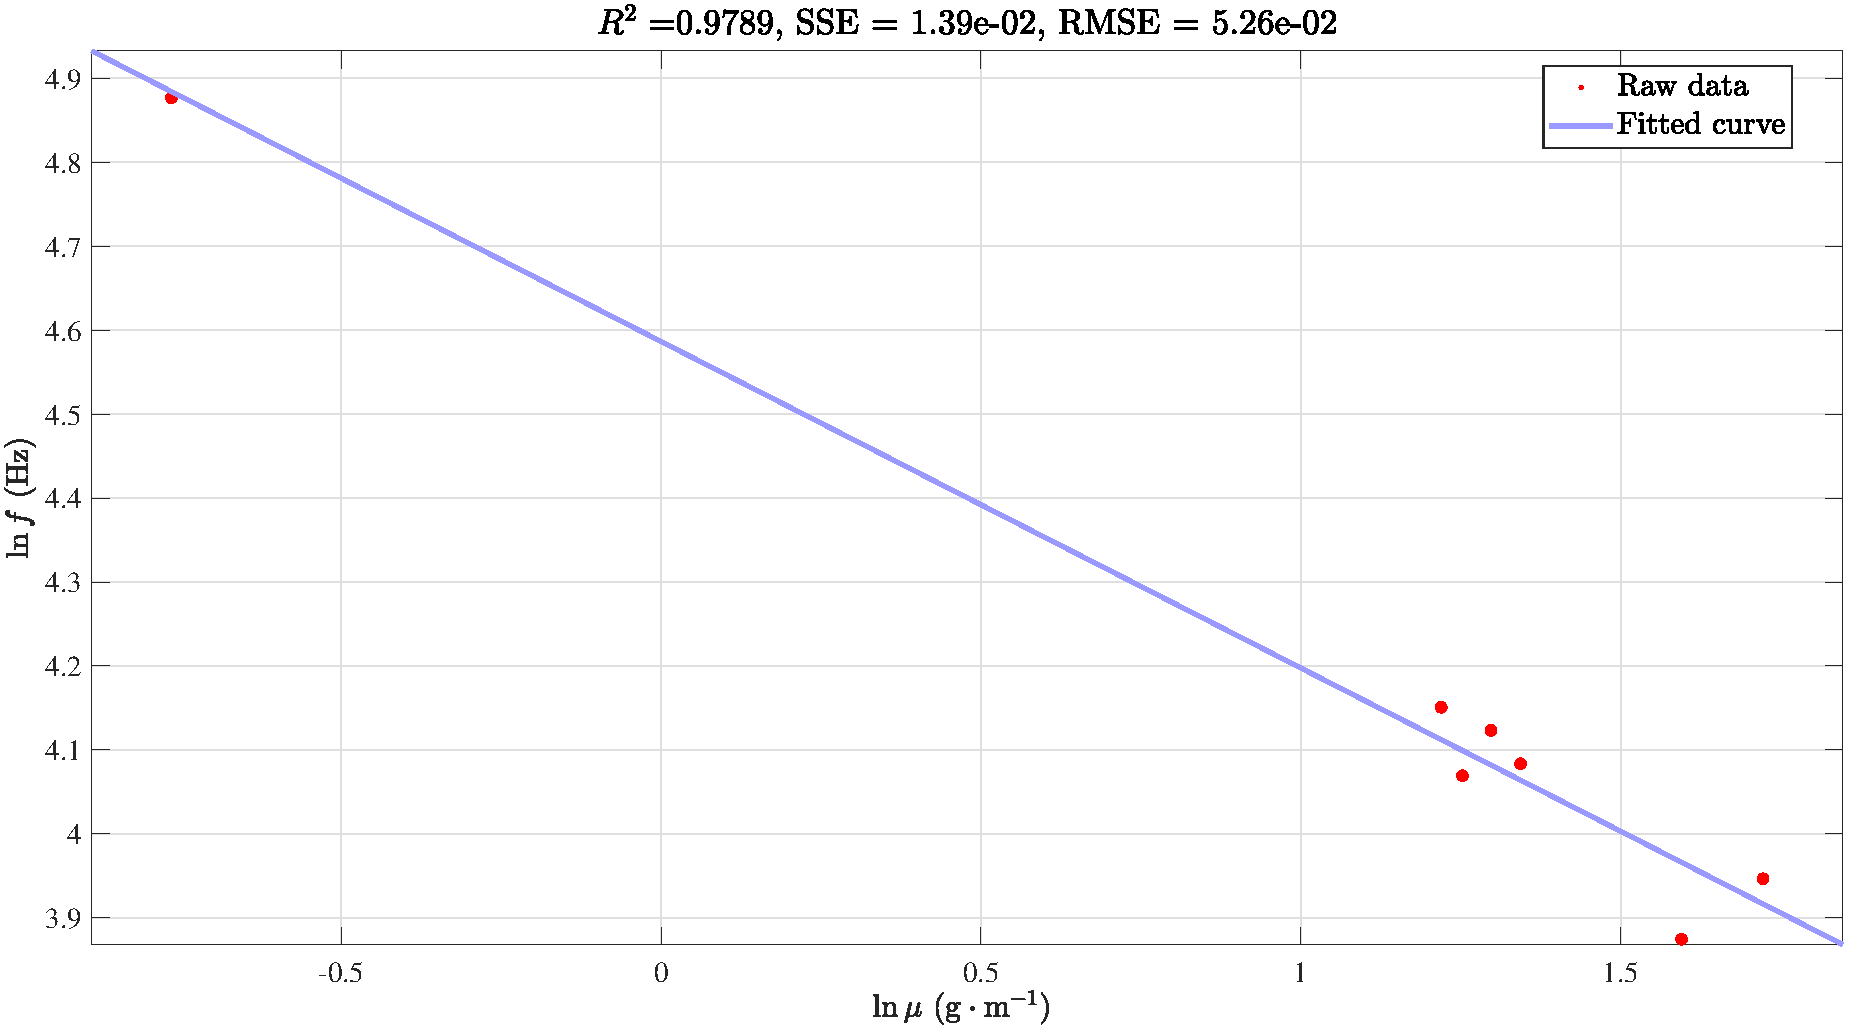
\includegraphics[width=12cm]{5.png}
    \caption{微波偏振实验:数据制图}
\end{figure}

\begin{center}
    \begin{tcolorbox}[colback=gray!10,%gray background
                      colframe=black,% black frame colour
                      width=5cm,% Use 8cm total width,
                      arc=1mm, auto outer arc,
                      boxrule=0.5pt,
                     ]
  微波偏振实验:实验总结
    \end{tcolorbox}
\end{center}

为了更清楚地记录数据变化,我将起始处的强度调整为193.9 mV(最大也只有200 mV)。
可以看到,在$\theta=30-70$度范围内,数据偏差还是比较大的。
经过询问刘老师,以往同学所作的这一实验数据都会相较于理论值偏小。
我认为误差的产生原因是最开始发生器和接收器就有微小夹角,并且二者的面并不是严格对准且垂直于实验桌面的——实验中我发现,细微的夹角变化就可以产生几毫伏甚至几十毫伏的浮动,非常敏感!

实验结果只能说初步验证了微波的马吕斯定律。



















\newpage

\section{思考题}

*这一部分回答实验讲义上的思考题,并融入一些我自己查阅到的资料。

\begin{enumerate}
    \item 思考题1:  \textbf{各实验内容主要误差影响是什么?}

(1)实验环境状态:实验的封闭性不佳,且环境不对称——一边有吸波材料的阻隔,另一边则较为空旷,不同的质地材料将会导致反射的微波干扰实验,影响测量结果,造成一定误差。
另外操作者的动作变化(比如移动、调节载物台等操作)或者同学老师经过实验台前,都会引起微波接受器显示屏的示数变化。

(2)微波试验仪器的局限:一是试验仪上的两个喇叭的对正关系,以及微波与单缝、双缝、反射板是否正交几乎只能靠目测调节,人为主观判断的因素较多;二是在部分实验进行的过程中,示数显示较不稳定(实际上发射的微波也不完全稳定),或者出现0或者很接近0的极小值的情况而导致无法分辨;三是
喇叭的固定并不是很稳固,可能会因为误触甚至碰到海绵等就会发生偏移,甚至于这种偏移还是人眼无法观测到的,且即使观测到了也无法迅速且有效地调整过来,就容易导致难以找到原因的误差。此外,有些缝或者板的固定性也较差。
四是微波波长(3.1915cm)和实验室中很多物品的尺寸量级相近,容易发生干涉、衍射等复杂的相互作用,干扰实验测量,影响测量结果。

(3)双缝干涉实验误差来源:双缝缝宽、双缝间距的尺度误差,双缝板面与几何
平面不完全相同(有所弯曲,应该是存储环境不好导致的问题),双缝干涉板发现与发射喇叭、接收喇叭轴线不完全同向等。

(4)迈克尔逊干涉实验误差来源:两个反射板不完全垂直,玻璃板不能恰好正对 45°方
向。此外,如果在测量过程中向两侧都移动了反射板,则会产生一定的滞后,产生回程差,
造成微波的测量误差。刻度尺读数不精确也会带来测量误差。

(5)布拉格衍射实验误差来源:模拟晶体本身和晶体材料结构并不完全相同,包括晶体小球不能做到完全规整排列,模
拟晶体外壳对微波的传播有干扰,细线对微波的传播有干扰,以及反射角入射角测量的误差。
(110)晶面实验中,即便将微波发射强度调至最大,微波接收器读数也较小,很大一部分原
因来自模拟晶体外壳对微波的阻挡等。

(6)单缝衍射实验误差来源:单缝并不完全处于双缝面上,金属板有一定的弯曲,单缝的中心不一定处于载物圆台的中
心,单缝宽度有误差,极小点附近光强过小,导致难以找到真正的最小点等。

(7)微波偏振实验误差来源:
微波试验仪仪器姿态并不完全标准,
反射、折射信号的影响等。

    \item 思考题2:  \textbf{金属是一种良好的微波反射器。其它物质的反射特性如何?是否有部分能量透过这些物质还是被吸收了?比较导体与非导体的反射特性。}

    微波照射在物体表面会有三种现象:透射、反射和吸收。

对于玻璃、塑料和瓷器等绝缘体,微波几乎是直接透射而非吸收;
而对于水和食物等极性分子就会吸收微波而使自身发热,
(这就是微波炉的基本原理)。
而对于金属类物质,则会反射微波。

微波透入介质时,由于损耗,
微波的部分能量会被介质吸收。
介质对微波的吸收主要由其介质损耗因数来决定。
介质的损耗因数与其对微波的吸收能力成正相关关系。

微波的能量较小,导体的电导率大,所以折射率高、反射率高,但非导体反射率不高,
所以微波会穿透物质或者被物质吸收从而发热。二者对长波的反射有较大差异,但一般而言,
导体反射能力更强一些。
值得一提的是,在分析导体对电磁波的反射时,
推导菲涅尔公式时的边界条件已不再适用,
但结合更细致的理论可以大致得出导体对微波的反射能力比非导体强的结论。

    \item 思考题3:  \textbf{为避免每台仪器微波间的干扰,使用吸波材料对每套设备进行了微波屏蔽,请问吸波材料的工作机理是什么?与屏蔽微波波长的关系是什么?}

吸波材料是指能吸收投射到其表面的电磁波能量,
并通过材料的介质损耗使电磁波能量转化为热能或其他形式的能量的材料,
其一般由基体材料(或粘接剂)与吸收介质(吸收剂)复合而成。
由于各类材料的化学成分和微观结构不同,吸波机理也不尽相同。
尽管如此,材料的吸波性能还是可以用宏观的电磁理论进行简要分析。
事实上,工程上也常常使用材料宏观的介电常数和磁导率来评价
吸波材料的反射和传输特性。材料吸收电磁波的基本条件是:

一、电磁波入射到材料上时,
它能尽可能反射而最大限度地进入材料内部,即要求材料满足阻抗匹配;

二、进入材料内的电磁波能迅速地几乎全部衰减掉,
即要求材料满足衰减匹配。吸波材料吸波与屏蔽微波的波长无关。

吸波材料的性能还与其外形有关,吸波的尖劈长度应与需屏蔽微波波长近似相等,以期
实现对微波的多次反射。

    \item 思考题4:  \textbf{假如预先不知道晶体中晶面的方向,是否会增加实验的复杂性?又该如何定位这些晶面?}

会增加实验的复杂性。如果不知道晶面法线方向,无法转动载物圆台对准刻线位置以标
定入射角和反射角,也就无法对应记录数据和所处角度。一般需要在实验前先确定晶面的位
置,才能进行进一步的测量,除了步骤上的增加,也带来了额外的误差。

定位晶面的一般方法是在合适的入射强度下,固定晶体和发射臂的位置,旋转反射臂扫
描晶体,确定诸极大值点处的两臂夹角,由此可以得到极大值点处的入射角和反射角。理论
计算可以得到此处的晶面间距,结合晶格常数可以得到此时可能的晶面指数。特别地,反射
强度最大的晶面是(100)面。

或者可以采用更为先进的实验仪器和技术手段,更加方便精确地定位晶面。

\end{enumerate}

\section{感想总结}


本次实验采用频率9.4GHz、波长 3.1893cm的微波,使用 DHMS-1 型微波光学综合实
验仪,成功地完成了收发喇叭的调试、对准,在此基础上,绘制出双缝干涉强度、模拟布拉
格衍射强度随角度变化的图线,测定了峰值的位置和强度、测定了模拟晶体的晶格常数,并
与理论值相比较,以较好的精确度验证了双缝干涉规律、布拉格公式。特别地,本次实验还
通过简易的迈克尔逊干涉装置,较为精确地测量了微波的波长,并以此验证了迈克尔逊干涉
规律。除此之外,我还完成了选做的两个实验:微波单缝衍射实验以及检验偏振的马吕斯定律,并且较好地验证了其基本规律。
关于每一部分具体的实验感想总结,可参考上述子实验报告的末尾。

除去上文已经提到的内容之外,我还产生了一些感想,总结如下:

·“打铁还需自身硬”。在正式做实验之前,必须先做好预习工作。
比如此次实验之前,我先完成了预习实验报告的撰写,对实验整体情况有了一个大概了解。在理解原理的基础上计算了部分实验的理论值,后者指导了我实验过程中的一些操作和判断。
在后续处理数据的时候,也提高了我的效率。
本次实验报告的撰写依赖于我新配置的\LaTeX 环境,以及Excel处理数据及绘制图像的功能。
此外,为了尽可能减小读取图像数据点造成的二次实验误差,我利用了Get Data软件进行了图像分析与读取操作。


·其次,要认真对待误差分析,分析其中原因。不能仅仅亦步亦趋,
按照标准操作动手,还要去想为什么。这次实验测量的数据较多,
需要整理、总结的部分也很多,这就很需要我们对误差分析的水平。
误差产生的原因以及怎么做才能减少误差,是我们都必须要去正视、去思考的问题。

·体悟理论与实验相结合的物理魅力。归根结底,物理是一门实验学科,对它的学习如果只
是从书本上看,从课堂上听,而没有动手亲自“学”的话,终究对其的理解和把握是有限的。在此之前,我对微波的布拉格衍射等相关概念已
经有所了解,但真正像这样动手测量一遍并绘制相关图像的过程中,我相信对它们的认识又加深了一层。


\bigskip
——————————

附:

1、预习实验报告(手写pdf版导入)

2、原始实验数据记录表(包含老师签名)(扫描为pdf版导入)

\newpage

\includepdf[pages={1-2}]{草稿.pdf}
\includepdf[pages={1-3}]{扫描全能王 2023-11-21 23.05.pdf}



\end{document}